\section{Modello del Dominio}
% XXX FEDE XXX %
%TODO i componenti alla larga (overview)

Questa sezione descriverà la composizione del nostro progetto alla luce di ciò che è già stato fatto e ciò che vogliamo introdurre.
Il progetto ha come priorità l'esecuzione di un brano improvvisato da parte di più musicisti, i quali non hanno (almeno per il momento) alcuna coscienza della presenza di altri musicisti.
Come mostrato in figura ~\ref{fig:dom}, la struttura del sistema consta di alcuni componenti differenti, che descriveremo nelle sezioni seguenti, organizzati esattamente come in un'orchestra reale (fatta eccezione per il player):
il direttore d'orchestra trasferisce le proprie informazioni generali riguardo all'esecuzione a un numero arbitrario di musicisti, i quali eseguono una parte definita del brano e la passano ad un player, che si occupa di riprodurre le composizioni dei musicisti.
I musicisti producono musica in un linguaggio che non è direttamente riproducibile dai sintetizzatori software, per questo è necessaria l'introduzione del player che traduce in maniera trasparente la rappresentazione interna in musica digitale in formato MIDI, differenziandosi da musicisti e direttore che sono da considerarsi agenti intelligenti (come verrà descritto più in dettaglio nei prossimi capitoli).

\begin{figure}[H]
\centering
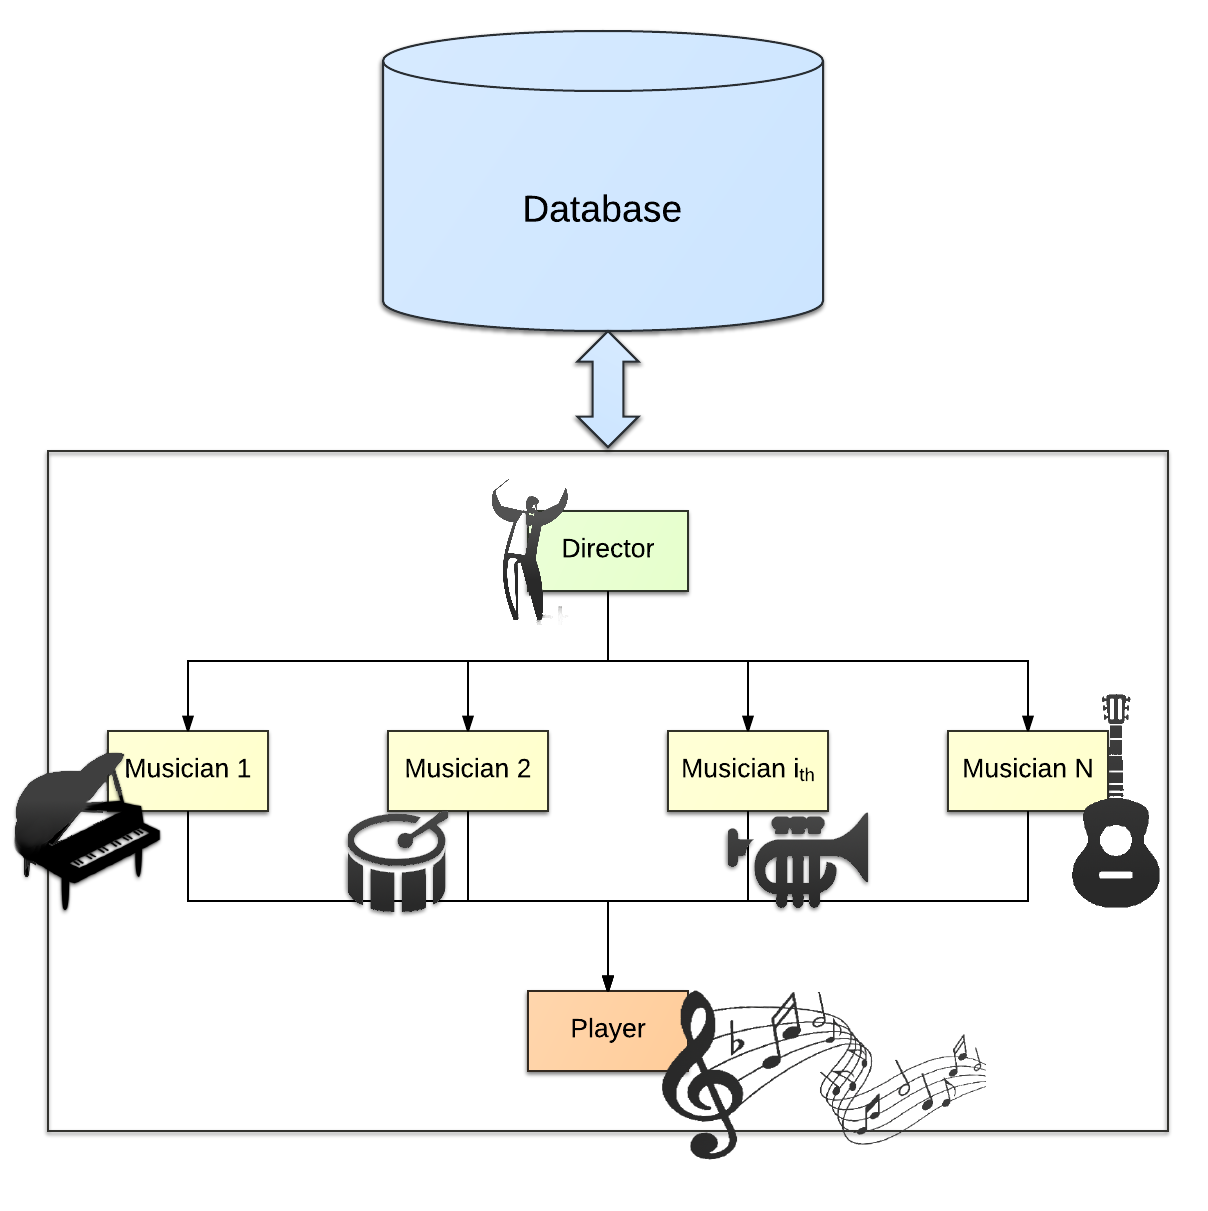
\includegraphics[scale=0.30]{img/model.png}
\caption{Schema dello scenario di progetto}
\label{fig:dom}
\end{figure}

Tali agenti operano in un ambiente con le seguenti proprietà che potremmo descrivere con la notazione PEAS;
\begin{itemize}
 \item Parzialmente osservabile, poiché i musicisti conoscono solo lo stato corrente del direttore, ovvero soltanto ciò che esso decide di far suonare più, ovviamente, il proprio stato, ma non conosce ciò che gli altri musicisti eseguono.
 Inoltre, il direttore non conosce lo stato interno dei musicisti, ma si limita a decidere i parametri della misura seguente mediante un proprio algoritmo interno.
 Questo aspetto è presente in parte per semplificare la struttura attuale, ma potrebbe essere in seguito modificato.
 \item Strategico, poiché lo stato successivo dell'ambiente non è determinato dalle mosse di un agente, ma deve tener conto anche delle mosse degli altri agenti, che, pur essendo cooperativi, potrebbero risultare imprevedibili.
 Il direttore decide le proprie mosse che influenzano la globalità del sistema, ma non ha controllo su ogni singolo agente.
 \item Episodico nel caso del musicista\footnote{L'implementazione probabilistica del musicista è completamente episodica, mentre la versione genetica è parzialmente episodica, in quanto non tiene conto delle sessioni di improvvisazione precedenti, ma ha carattere sequenziale all'interno di una singola esecuzione.}, poiché le azioni intraprese da quest'ultimo non hanno ripercussioni future né costituiscono un parametro di decisione nell'episodio seguente.
 La percezione del musicista è definita dalle informazioni pervenute dal direttore.
 Nel caso del direttore invece l'ambiente assume una connotazione sequenziale, poiché alcuni parametri dell'azione corrente determinano una probabilità di passaggio a differenti azioni successive possibili.
 \item Statico, poiché solo gli agenti coinvolti possono variare l'ambiente.
 \item Discreto, poiché, pur operando in un'ottica real-time, le azioni degli agenti si basano su unità di tempo atomiche uguali per tutti, come del resto impone la teoria musicale.
 \item Multiagente, anche se le interazioni reali fra agenti sono relativamente scarse. Questo fa di un ambiente concettualmente cooperativo, in realtà un ambiente composto da unità che dagli altri agenti possono essere viste come stocastiche e imprevedibili.
 \end{itemize}

%https://www.lucidchart.com/documents/edit/67c03865-48ea-4f6a-b052-e9f9c4cd8196?
